%-------------------------
%clang
%(c) H.Buchmann FHNW 2008
%export TEXINPUTS=.:${HOME}/fhnw/edu/:${HOME}/fhnw/edu/tinL/config/latex:${HOME}/fhnw/edu/config//:
%-------------------------
\documentclass{beamer}
\usepackage{beamer}
%---------------------
%local defines
%(c) H.Buchmann FHNW 2009
%$Id$
%---------------------
\newcommand{\target} {\beaglebone\xspace}
\newcommand{\targetS}{{\bf BBG}\xspace}
\newcommand{\host}   {{\em Host}\xspace}
\newcommand{\targetroot} {{\bf target-root}\xspace}
\newcommand{\kernel} {{\bf kernel}\xspace}
\renewcommand{\c}{{\bf C}\xspace}
\newcommand{\cpp}{{\bf C++}\xspace}
\newcommand{\posix}{{\bf POSIX}\xspace}

\input{/home/buchmann/latex/dirtree/dirtree.tex}

\usepackage[absolute]{textpos}
\setlength{\TPHorizModule}{1mm}
\setlength{\TPVertModule}{1mm}

\begin{document}

\title[Build]{Ein ganzes \linux}

\frame{\titlepage}

\begin{frame}{Um was geht es ?}
 \begin{itemize}
  \item ein \linux von Grund auf bauen
  \begin{itemize}
   \item nicht meht so schwer wie auch schon
  \end{itemize}
  \item nicht v�llig automatisiert
  \item Alternative zu {\bf yocto} \& Co.
 \end{itemize}
\end{frame}

\begin{frame}{Ziel}{\linux auf dem \target}
\begin{itemize}
 \item command based
 \item Ethernet
 \item \cod{ssh} 
 \item \cod{sshfs}
 \item moderne Toolchain inkl. {\em c++11} \cpp 
\end{itemize}
\end{frame}

\section{Die Komponenten}
\begin{frame}{Komponenten}{\target und \host}
 \begin{block}{\target}
  \begin{description}
   \item[Kernel] ein File
   \item[root] ein Filesystem
  \end{description}
 \end{block}
 \begin{block}{\host}
  \begin{description}
   \item[Toolchain] binutils, gcc
  \end{description}
 \end{block}
\end{frame}
\subsection{Target \target}

\begin{frame}{�bersicht}
 \begin{center}
  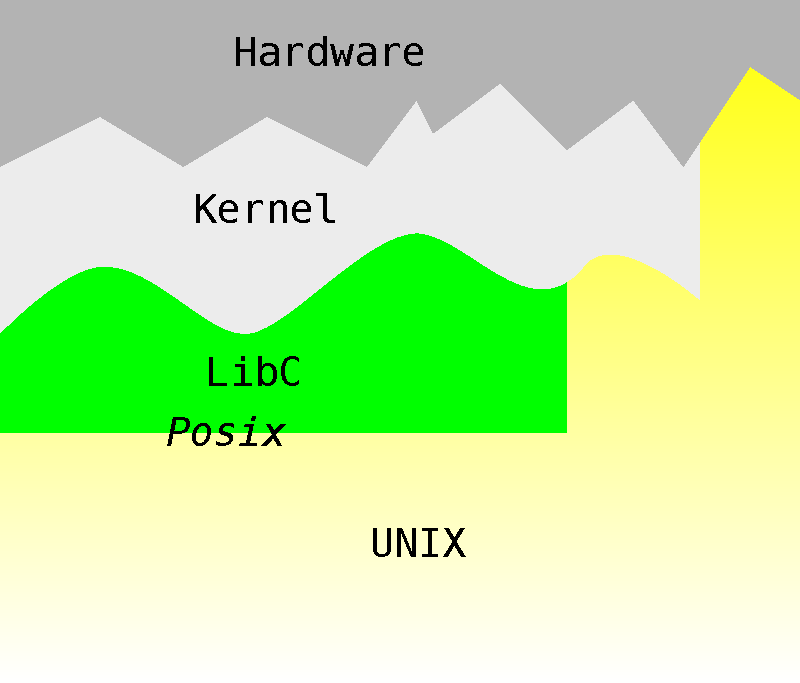
\includegraphics[width=8cm]{layers.pdf}
 \end{center}
\end{frame}

\begin{frame}{Die Komponenten}{f�r \raspberry}
 \begin{description}
  \item[Hardware] \raspberry
  \item[Kernel] zugeschnitten auf \raspberry
  \begin{itemize}
    \item {\tiny \url{https://github.com/raspberrypi/linux.git}}
  \end{itemize}	
  \item[root] das Filesystem
  \begin{description}
   \item[LibC] eglibc 
   \begin{itemize}
    \item {\tiny \url{http://www.eglibc.org/home}}
   \end{itemize}	
   \item[\unix] busybox
   \begin{itemize}
    \item {\tiny \url{http://www.busybox.net/}}
   \end{itemize}
   \item[...] Weitere \unix basierte Komponenten
   \begin{itemize}
    \item das \cod{configure}, \cod{make}, \cod{make install} Triple 
   \end{itemize}
   \end{description}
 \end{description}
\end{frame}

\subsection{\host}
\begin{frame}{Toolchain}
 \begin{description}
  \item[binutils] linker \& Co.
  \item[gcc] compiler
  \begin{itemize}
   \item \cod{libgcc} die Bibliothek f�r den Compiler
  \end{itemize}
 \end{description}
 
 \begin{remarks}
 \item die Toolchain muss zweimal gebaut werden
 \begin{itemize}
  \item f�r den \kernel und \cod{libc} 
  \item f�r \unix/\posix
 \end{itemize}
 \item das target
 \begin{itemize} 
  \item \cod{cpu-vendor-os}
  
 \end{itemize}
 \end{remarks}
\end{frame}

\begin{frame}{Die Verzeichnisstruktur}
\dirtree{%
 .1 .
 .2 scripts.
 .3 common.h \DTcomment{used in (all) scripts}.
 .2 config.
 .3 Makefile.
 .2 build \DTcomment{home of the build files}.
 .2 target-root.
 .2 target-mount.
 .2 tc \DTcomment{the new toolchain}.
 .2 src \DTcomment{own programs}.
 .2 work.
 .3 $\to$ {../config/Makefile}.
}
\end{frame}

\section{Build}
\begin{frame}{Build}{die Schritte 1}
 \begin{itemize}
  \item \cod{binutils}
  \item \cod{gcc-bare} 
  \item \cod{kernel} mit ein paar {\em rules}
   \begin{itemize}
    \item \cod{bcmrpi\_defconfig}
    \item \cod{zImage}
    \item \cod{headers\_install}
   \end{itemize}
   
  \item \cod{eglibc} 
  \item \cod{gcc} 
  \item Test
  \begin{itemize}\item im Verzeichnis \cod{work}\end{itemize}
 \end{itemize}
\end{frame}

\begin{frame}{Build}{die Schritte 2}
 \begin{itemize}
  \item \cod{busybox}
  \begin{itemize}
   \item Installation auf SD-Card
   \item \cod{fakeroot}
  \end{itemize}
  \item \cod{openssh} die volle Implementation 
  \begin{itemize}
   \item \cod{zlib}
   \item \cod{openssl}
   \item \cod{openssh}
  \end{itemize}
  \item \cod{sshfs}
 \end{itemize}
\end{frame}


\begin{frame}{Skripts und Argumente}{initiales System}
 \begin{tabular}{lll}
  \cod{binutils.sh}\\
  \cod{gcc-bare.sh}& &kernel libc\\
  \cod{kernel.sh}  & \cod{bcmrpi\_defconfig}\\
                   & \cod{zImage}\\
                   & \cod{headers\_install}\\
  \cod{eglibc.sh}  &\\
  \cod{gcc.sh}     &&C/C++ POSIX\\
  \cod{busybox.sh} &busybox\\
  		   &install\\
  \cod{target-root.sh}
 \end{tabular}
\end{frame}

\begin{frame}{Target}{erster Versuch}
\begin{itemize}
 \item transfer auf SD Karte
 \item Internet
\end{itemize}
\end{frame}

\begin{frame}{Skripts und Argumente}{ssd}
\begin{tabular}{lll}
 \cod{zlib.sh}\\
 \cod{openssl.sh}&&die kryptographischen Algorithmen\\
 \cod{openssh.sh}
\end{tabular}
\end{frame}

\begin{frame}{Target}{ssh}
\begin{itemize}
 \item \cod{ssh}
 \item \cod{sshd}
 \item Keys
\end{itemize}
\end{frame}

\begin{frame}{sshfs}{funktioniert noch nicht}
 \begin{itemize}
  \item Die Bibliothek \cod{glib}
  \item Ersatz
  \begin{itemize}
   \item \cod{sftp}
  \end{itemize}
 \end{itemize}
\end{frame}

\section{Modules}
\begin{frame}{Modules}
\begin{itemize}
 \item siehe \cod{6-modules}
\end{itemize}
\end{frame}

\begin{frame}{Modules}{Verzeichnisstruktur}
\begin{block}{Host}
\dirtree{%
 .1 BUILD\_HOME.
 .2 modules.
 .3 Makefile \DTcomment{for own modules}.
 .3 *.{c/h} \DTcomment{the own sources}.
 .2 scripts.
 .3 module.sh.
}
\end{block}
\begin{block}{\target}
\dirtree{%
.1 /.
.2 work.
}
\end{block}
\end{frame}
\begin{frame}{Herstellung}{Workflow}
 \begin{block}{Host}
 \begin{itemize}
  \item \cod{sh scripts/module.sh {\em module}}
  \item \cod{scp}, \cod{sftp}, \cod{ftp}
 \end{itemize}
 \end{block}
 \begin{block}{\target}
  \begin{itemize}
   \item \cod{insmod}
   \item \cod{rmmod}
  \end{itemize}
 \end{block}
\end{frame}

\end{document}
